\section{HIO as graphical criterion}

Consider a dynamic system with matrices $A$, $B$, $C$ and $D$ with $n$ state variables, 
$p$ observables and $m$ hidden inputs. As before we neglect the known inputs via $B$. 
Now assume each hidden input affects only one state variable directly and we observe only 
single state variables, i.e.
\begin{equation}
	D = \begin{pmatrix}
	 e_{i_1} & e_{i_2} & \hdots &  e_{i_m}
	\end{pmatrix} \tab {and}
	C = \begin{pmatrix}
	e_{j_1} & e_{j_2} & \hdots & e_{j_p}
	\end{pmatrix}^\text{T}
\end{equation}
where $e_i$ denotes the $i$-th canonical vector of length $n$. Without loss of generality 
we can assume that $i_1<i_2<\ldots < i_m$ and $j_1<j_2<\ldots < j_p$. Furthermore we can 
identify $D$ and $C$ with the sorted index sets $\hat{D}=\{i_1,\ldots,i_m\}$ and 
$\hat{C}=\{j_1,\ldots,j_p\}$, respectively.

\begin{definition}{}{}	
	We call a system \textit{structural hidden input observable} if almost each systems 
	that we can create by changing the numerical values of the nonzero elements of $A$ are 
	hidden input observable.
\end{definition}

We will derive a theorem of the form:\\

	A system is structural hidden input observable, if each input knot has its own 
	observed knot such that there is a shortest path from input to output knot that 
	includes no other input knots.\\
	
Before we can prove this we have to make some definitions and prove some graph theoretical 
lemmas.

\subsection{Basics of Graph Theory}

\begin{definition}{Graphtheoretical Definitions}{}
\begin{enumerate}
	\item
	When we consider a dynamic system as network, the state variables $x_i$ shall be called 
	\textit{knots}.
	\item	
	Let $A$ be the matrix of the linear dynamic system. The \textit{path factor} of a 
	sequence $\pi=(x_{l_0},x_{l_1},\ldots,x_{l_N})$ is
	\begin{equation}
		F(\pi):=\prod\limits_{i=0}^{N-1} A_{l_{i+1}l_i} \quad . 
	\end{equation}
	\item
	We define a relation
	\begin{equation}
	x_a \sim x_b \quad \overset{ { \text{definition} } }{ \Longleftrightarrow } 
	F( (x_a,x_b) )\neq 0  \quad \left( \quad \Longleftrightarrow \quad A_{ba} \neq 0 \quad 
	\right)\quad .
	\end{equation}
	\item
	A \textit{path} from $x_a$ to $x_b$ is a sequence $(x_{l_0},x_{l_1},x_{l_2},
	\ldots,x_{l_N})$ with indices $l_i$ such that 
	\begin{equation}
	x_{l_0} = x_a \tab{,} x_{l_N} = x_b \tab{and} x_{l_i} \sim x_{l_{i+1}}	\quad .
	\end{equation}
	\item
	The \textit{length} of such a path is $||(x_{l_0},\ldots, x_{l_N} )||=N$. 
	\item	
	\begin{enumerate}
	\item
	For the \textit{set of all paths} from $x_a$ to $x_b$ we write $\Gamma(x_a,x_b)$.
	\item
	The \textit{set of paths of length $k$} from $x_a$ to $x_b$ is $\Gamma_k(x_a,x_b)$.
	\item
	For the \textit{shortest path} from $x_a$ to $x_b$ (if it exists) we write 
	$\gamma(x_a,x_b)$.
	\end{enumerate}
	\item
	The \textit{distance} between $x_a$ and $x_b$ is $d(x_a,x_b):=||\gamma(x_a,x_b)||$ if 	
	it exists. If there is no path from $x_a$ to $x_b$ we write $d(x_a,x_b)=\infty$.
	\item
	 \begin{enumerate}
	\item		
	The path $(x_a)$ is called \textit{trivial path}. 
	\item	
	The path $(x_a,x_a)$ is called \textit{self-loop}. 
	\item	
	Any path $(x_a,x_{l_1},\ldots,x_{l_{N-1}},x_a)$ is called 
	\textit{loop}. 
	\end{enumerate}
	\item	
	Let $\pi$ and $\pi'$ be paths. 
	\begin{enumerate} \item
	We write $x_i\in\pi$ if $x_i$ appears in $\pi$.
	\end{enumerate}
\end{enumerate}	
\end{definition}

\begin{definition}{}{}
	Let $\pi = (x_{l_0},\ldots,x_{l_N})$ and $\pi' = (x_{k_0},\ldots,x_{k_N'})$ be 
	sequences of knots.
	\begin{enumerate}
	\item 
	\begin{equation}
	\pi \odot \pi' := (x_{l_0},\ldots,x_{l_N},x_{k_0},\ldots,x_{k_N'})
	\end{equation}
	\item If $x_{l_N}=x_{k_0}$.
	\begin{equation}
	\pi \oplus \pi' := (x_{l_0},\ldots,x_{l_N},x_{k_1},\ldots,x_{k_N'})
	\end{equation}	
	\item
	We write 
	$\pi \subset \pi'$ if $\pi'=(x_{l_0},\ldots,x_{l_{N'}} ) \oplus \pi \oplus 
	(x_{l_{ N'+||\pi||} },\ldots,x_{l_N})$.
	\end{enumerate}
\end{definition}

\begin{lemma}{}{}
	\begin{enumerate}
	\item The path factor is a homomorphism, i.e. 
	\begin{equation}
	F(\pi\oplus \pi') = F(\pi) F(\pi') 
	\end{equation}	
	and 
	\begin{equation}
	F(\pi \odot \pi') = F(\pi) F( (x_{l_N},x_{k_0}))F(\pi') \quad . 
	\end{equation}
	\item For a sequence $\pi=(x_{l_0},\ldots,x_{l_N})$
	\begin{equation}
	F(\pi) \neq 0 \quad \Leftrightarrow \quad \text{ $\pi$ is a path} \quad .
	\end{equation}
	\end{enumerate}
\end{lemma}
\begin{proof}
	\begin{enumerate}
	\item
	Write down the definitions to see that these equations hold.
	\item
	Decompose $\pi = (x_{l_0},x_{l_1})\oplus (x_{l_1},x_{l_2})\oplus \ldots $ to see that 
	\begin{equation}
	F(\pi) = \prod\limits_{i=0}^{N-1} F(x_{l_{i}},x_{l_{i+1}}) = \prod\limits_{i=0}^{N-1}
	A_{l_{i+1}l_i} \quad .
	\end{equation}
	If and only if all factors $A_{l_{i+1}l_i}\neq 0$, then by definition $\pi$ is a path.
	\end{enumerate}
\end{proof}

\clearpage
\begin{lemma}{}{}
	Let $\pi$ be a path from $x_a$ to $x_b$.
	\begin{enumerate}
	\item For two paths $\pi$ and $\pi'$, $||\pi||+||\pi'|| = ||\pi\oplus \pi'||$. \\
	\textit{(Addition of path lengths)}
	\item If any $x_i$ appears more than once in $\pi$, then 
	$ \pi \neq \gamma(x_a,x_b)$. \\
	\textit{(Shortest paths contain no loops)}
	\item If there are $x_{l_i}, x_{l_j} \in \pi$ such that $x_{l_i}\sim x_{l_j}$ and 
	$j\neq i+1$,\\ then $\pi\neq \gamma(x_a,x_b)$.\\
	\textit{(No shortcuts for shortest paths)}
	\item Let $x_a$, $x_b$ ,$x_{a'}$ and $x_{b'}$ be knots. If $\pi$ is a path from 
	$x_{a'}$ to $x_{b'}$ and if $\pi\subset \gamma(x_a,x_b)$ then $\pi = \gamma(x_{a'},
	x_{b'} )$.\\
	\textit{(Subpaths of a shortest path are again a shortest path)}
	\end{enumerate}
\end{lemma}
\begin{proof}
	\begin{enumerate}
	\item Consider two paths $\pi = ( x_{l_0},\ldots,x_{l_N} )$ and $\pi'= (x_{k_0},\ldots,
	x_{k_{N'} } ) $ with the property $x_{l_N} = x_{k_0}$. Then 
	$\pi\oplus \pi' = (x_{l_0},\ldots,x_{l_N},x_{l_{N+1}},\ldots, x_{N+N'})$ with 
	$l_{N+i} = k_i$. We see that $||\pi||=N$, $||\pi'||=N'$ and $||\pi\oplus \pi'||=N+N'$.
	\item Assume $x_{l^*}$ appears twice in a path $\pi$ from $x_a$ to $x_b$. 
	Then we can write $\pi = \pi_1 \oplus \pi^* \oplus \pi_2$ such that $\pi_1$ is a 
	path from $x_a$ to $x_{l^*}$, $\pi^*$ is a nontrivial path from $x_{l^*}$ to $x_{l^*}$ 
	and $\pi_2$ is a path from $x_{l^*}$ to $x_b$. Thus also $\pi_1\oplus \pi_2$ is a path 
	from $x_a$ to $x_b$ and $||\pi_1\oplus\pi_2|| = ||\pi||-||\pi^*||$ which means $
	\pi_1\oplus \pi_2$ is shorter than $\pi$ and therefore $\pi$ cannot be the shortest 
	path $\gamma(a,b)$.
	\item We can write $\pi = \pi_1 \oplus \pi_2 \oplus \pi_3$ such that $\pi_1$ is from 
	$x_a$ to $x_{l_i}$, $\pi_2$ is from $x_{l_i}$ to $x_{l_j}$ and $\pi_3$ is from 
	$x_{l_j}$ to $x_b$. Since $x_{l_i}\sim x_{l_j}$ we can define 
	$\pi^* = \pi_1 \oplus (x_{l_i},x_{l_j})\oplus \pi_3 $. We see that 
	$||\pi^*||\leq ||\pi||$ and equality holds only if $||\pi_2||=1$ which means that 
	$l_j =l_{i+1}$ or equivalently $j=i+1$. Thus if $j\neq i+1$ we have found a shorter 
	path and  $\pi$ cannot be $\gamma(a,b)$.
	\item We can write $\gamma(x_a,x_b) = \pi_1 \oplus \pi \oplus \pi_2$ where $\pi_1$ is 
	from 
	$x_a$ to $x_{a'}$ and $\pi_2$ is from $x_{b'}$ to $x_b$. Now assume $\pi \neq 
	\gamma(x_{a'},x_{b'})$. Then $\pi^* = \pi_1\oplus \gamma(x_{a'},x_{b'}) \oplus \pi_2 $ 
	is shorter than $\gamma(x_a,x_b)$. This is in contradiction to the assumptions. 
 	\end{enumerate}
\end{proof}

\clearpage

\subsection{Structural Dynamic Networks}
Now we prove some lemmas to connect the rank conditions of reduced matrices with graphical 
properties.
%
%\begin{lemma}{}{}
%	Consider $\gamma(x_a,x_b) = (x_a=x_{l_0},x_{l_1},
%	\ldots,x_{l_{K-1}},x_{l_K} =x_b) $. Then
%	\begin{equation}
%	A^2_{l_{j}l_i} =\sum\limits_{\mu} A_{l_j \mu} A_{\mu l_i} =A_{l_j l_{i+1}} 
%	A_{l_{i+1} l_i}
%	  \left\{ \begin{matrix}
%	\neq 0 \tab{if } j=i+2 \\ = 0 \tab{else}
%\end{matrix}	\right. \quad .
%	\end{equation}
%\end{lemma}
%\begin{proof}
%	If there is a $\mu$ such that $x_{l_i}\sim x_\mu$ and 
%	$x_\mu\sim x_{l_j}$ then consider \\$\pi = \gamma(x_a,x_{l_i}) \oplus (x_{l_i},x_\mu, 
%	x_{l_j}) \oplus \gamma(x_{l_j},x_b)$. If and only if $\mu = l_{i+1} = l_{j-1}$ this is
%	consistent with $\gamma(x_a,x_b)$ being the shortest path. \\
%	
%	Consider $j=i+2$. Then by the above argument only $\mu = l_{i+1}$ leads to\\ 
%	$A_{l_j\mu}A_{\mu l_i} \neq 0$.\\
%	
%	Consider $j\neq i+2$. Then by the above argument for each $\mu$ we get \\ 
%	$A_{l_j\mu}A_{\mu l_i} =0$.
%\end{proof}

\begin{lemma}{}{}
	Let $k\in\mathbb{N}$ and $x_a$, $x_b$ knots of a network. We consider $A$ as a 
	structural matrix, i.e. we ignore special cases, in which different elements of 
	$A$ exactly neutralise each other. Then
	\begin{equation}
	A^k_{ba} \neq 0 \quad \Leftrightarrow \quad \exists \text{ a path from } x_a 
	\text{ to } x_b \text{ of length }k \quad .
	\end{equation}
\end{lemma}
\begin{proof}
	We write 
	\begin{equation}
	A^k_{ba} = \sum\limits_{l_1,l_2,\ldots,l_{k-1}=1}^n A_{b l_{k-1}} \ldots A_{l_2 l_1} 
	A_{l_1 a} = \sum\limits_{\pi\in\Gamma_k(x_a,x_b)} F(\pi)
	 \quad .
	\end{equation}		
	\begin{itemize}
	\item If $\Gamma_k(x_a,x_b)=\emptyset$ then $A^k_{ba}=0$ since there is nothing to sum.
	\item If $\Gamma_k(x_a,x_b)\neq\emptyset$ then there is at least one $F(\pi)\neq 0$ and 
	since we consider structural properties this is sufficient to show that $A^k_{ba}\neq 
	0$.
	\end{itemize}		
\end{proof}


\begin{lemma}{}{}
	Assume there exists a shortest path \\ 
	$\gamma(x_a,x_b) = (x_a=x_{l_0},x_{l_1},\ldots,x_{l_{K-1}},x_{l_K} =x_b) $ 
	from $x_a$ to $x_b$. \\
	Then for each $k \leq K $
	\begin{equation}
	A^\kappa_{l_k a}  = 0  \quad \text{if }\kappa <k \tab{and} A^k_{l_k a} \neq 0
	\quad .
	\end{equation}
\end{lemma}
\begin{proof}
	Note that each $\gamma(x_a,x_{l_k})\subset \gamma(x_a,x_b)$ hence it is a 
	shortest path of length $k$. \\
	\begin{itemize}
	\item
	Consider $\kappa < k$ and assume $A^\kappa_{l_k a}\neq 0$. Then by the previous 
	lemma there exists a path from $x_a$ to $x_{l_k}$ of length $\kappa <k=
	||\gamma(x_a,x_{l_k})||$, 
	which is not possible, since $\gamma(x_a,x_{l_k})$ already is the shortest path.
	 Therefore $A^\kappa_{l_k a}=0$.
	\item	
	Consider $\kappa = k$. Then we know that $\gamma(x_a,x_{l_k})$ is a path from 
	$x_a$ to $x_{l_k}$ of length $k$, thus by the previous lemma $A^k_{l_k a}\neq 0$.  
	\end{itemize}
\end{proof}


\clearpage
%
%\begin{proposition}{First nonzero column}{}
%	Choose one $a\in \hat{D}$ and assume that
%	\begin{equation}
%	b = \text{arg} \underset{b'\in\hat{D}}{\min} || \gamma(x_{a},x_{b'}) || 
%	\end{equation}
%	exists. Since $a\in\hat{D}$ we know that $a=i_\alpha$ and $b=j_\beta$. 
%	By construction the $\alpha$-th column of $D$ is $e_a$ and the $\beta$-th row of 
%	$C$ is $e_b^\text{T}$. \\
%	
%	Then for each $\kappa < ||\gamma(x_a,x_b)||$
%	\begin{equation}
%	(CA^\kappa D)_{\mu \alpha} = 0 \quad \forall \mu\in\{1,2,\ldots,p \}
%	\end{equation}
%	and if $\kappa=||\gamma(x_a,x_b)||$ at least the component $\mu=\beta$ is nonzero.
%\end{proposition}
%\begin{proof}
%	Let $x_a$ and $x_b$ be knots as defined above and $K:=||\gamma(x_a,x_b)||$.
%	We write down
%	\begin{equation}
%	(CA^\kappa D)_{\mu \alpha} = \sum\limits_{\lambda, \rho=1}^n C_{\mu\lambda} 
%	A^\kappa_{\lambda \rho} 
%	D_{\rho \alpha} \quad .
%	\end{equation}
%	Note that $D_{\rho\alpha}$ is the Kronecker-delta $\delta_{\rho a}$ and that 
%	the $\mu$-th row of $C$ is $e_{j_\mu}^\text{T}$, i.e. $C_{\mu \lambda} = 
%	\delta_{\lambda {j_\mu}}$, thus
%	\begin{equation}
%	(CA^\kappa D)_{\mu \alpha} = A^\kappa_{j_\mu a}  \quad .
%	\end{equation}
%	\begin{itemize}
%	\item
%	Consider $\kappa <k$ and assume there is a $\mu$ such that $A^\kappa_{j_\mu a}\neq 0$. 
%	Then there is a path from $x_a$ to the observed knot $x_{j_\mu}$ of length $\kappa$. 
%	This is in contradiction to $\gamma(x_a,x_b)$ being the shortest path from $x_a$ to an 
%	observed knot. Therefore $(CA^\kappa D)_{\mu\alpha}=0$.\\
%	\item
%	Now consider $\kappa = K$. Then the existence of $\gamma(x_a,x_b)$ ensures $A^k_{ba}
%	\neq 0$ and since we can choose $\mu=\beta$ which means $j_\mu = b$ we know 
%	that $A^k_{b a}\neq 0$ and therefore $(CA^kD)_{\beta\alpha}\neq 0$.
%	\end{itemize}
%\end{proof}
%
%
%\begin{proposition}{First nonzero row}{}
%	Choose one $b\in \hat{C}$ and assume that
%	\begin{equation}
%	a = \text{arg} \underset{a'\in\hat{D}}{\min} || \gamma(x_{a'},x_{b}) || 
%	\end{equation}
%	exists, i.e. there exists at least one path from at least the hidden input knot to the 	
%	observed knot $x_b$. Since $a\in\hat{D}$ we know that $a=i_\alpha$ and $b=j_\beta$. 
%	By construction the $\alpha$-th column of $D$ is $e_a$ and the $\beta$-th row of 
%	$C$ is $e_b^\text{T}$. \\
%	
%	Then for each $\kappa < ||\gamma(x_a,x_b)||$
%	\begin{equation}
%	(CA^\kappa D)_{\beta\mu} = 0 \quad \forall \mu\in\{1,2,\ldots,m \}
%	\end{equation}
%	and if $\kappa=||\gamma(x_a,x_b)||$ at least the component $\mu=\alpha$ is nonzero.
%\end{proposition}
%\begin{proof}
%	The proof is analogous to the latter proof. \\
%	
%	Let $x_a$ and $x_b$ be knots as defined above and $K:=||\gamma(x_a,x_b)||$.
%	We write down
%	\begin{equation}
%	(CA^\kappa D)_{\beta \mu} = \sum\limits_{\lambda, \rho=1}^n C_{\beta\lambda} 
%	A^\kappa_{\lambda \rho} 
%	D_{\rho \mu} \quad .
%	\end{equation}
%	Note that this time $C_{\beta\lambda}$ is the Kronecker-delta $\delta_{b \lambda}$ and 
%	that the $\mu$-th column of $D$ is $e_{i_\mu}^\text{T}$, i.e. $D_{\rho \mu} = 
%	\delta_{\rho {i_\mu}}$, thus
%	\begin{equation}
%	(CA^\kappa D)_{\mu \alpha} = A^\kappa_{b i_\mu}  \quad .
%	\end{equation}
%	\begin{itemize}
%	\item
%	Consider $\kappa <k$ and assume there is a $\mu$ such that $A^\kappa_{b i_\mu}\neq 0$. 
%	Then there is a path from the input knot $x_{i_\mu}$ to $x_b$ of length $\kappa$. 
%	This is in contradiction to $\gamma(x_a,x_b)$ being the shortest path from an input 
%	knot to $x_b$. Therefore $(CA^\kappa D)_{\beta\mu}=0$.\\
%	\item
%	Now consider $\kappa = K$. Then the existence of $\gamma(x_a,x_b)$ ensures $A^k_{ba}
%	\neq 0$ and since we can choose $\mu=\alpha$ which means $i_\mu = a$ we know 
%	that $A^k_{b a}\neq 0$ and therefore $(CA^kD)_{\beta\alpha}\neq 0$. 
%	\end{itemize}
%\end{proof}

\begin{proposition}{}{}
	Let $x_a$ and $x_b$ be a hidden input knot and an observed knot, respectively. We can 
	write $a=i_\alpha$ and $b=j_\beta$ for an $\alpha\in\{1,2,\ldots,m\}$ and 
	$\beta\in\{1,2,\ldots,p\}$.\\
	Then
	\begin{equation}
	(CA^kD)_{\beta\alpha} \neq 0 \quad \Leftrightarrow \quad \exists \text{ a path from }
	x_a \text{ to } x_b \text{ of length }k \quad . 
\end{equation}		
	As a corollary, assume $\gamma(x_a,x_b)$ exists and is of length $K$.
	\begin{equation}
	(CA^kD)_{\beta\alpha} = 0 \quad \text{for }k<K \tab{and} (CA^KD)_{\beta\alpha}\neq 0 
	\quad .
	\end{equation}
	
\end{proposition}
\begin{proof}
	We write as a sum
	\begin{equation}
	(CA^k D)_{\beta\alpha} = \sum\limits_{\lambda,\rho=1}^n C_{\beta \lambda} A^k_{\lambda
	\rho} D_{\rho \alpha} = A^k_{ba} \quad .
	\end{equation}
	Now we can simply apply lemma 7 and lemma 8 to finish the proof.
\end{proof}

With this proposition we are able to get the structure of the matrices $M_q$ by graphical criterions. As always 
we set the dimension of state space, observation space and hidden input space to be $n$, $p$ and $m$, 
respectively, and take a fixed integer $K$. Then the $\beta$-th row of $M_K$ reads
\begin{equation}
	\begin{bmatrix}
	\Gamma_0(x_{i_1},x_b) & \ldots &  \Gamma_0(x_{i_m},x_b)  & \dots  &
 	\Gamma_K(x_{i_1},x_b) & \ldots &  \Gamma_K(x_{i_m},x_b) 
	\end{bmatrix} \label{eq:M_q_beta}
\end{equation}
where $i_1,\ldots,i_m$ are the indices of $\hat{D}$ and $x_b$ is the associated knot of $\beta\in\hat{C}$. 
In the latter equation and henceforth we use the sets $\Gamma_k$ as 
indicators, i.e. it they represent the value $0$ if $\Gamma_k(x_{i,1},x_b)=\emptyset$ and $1$ if not.
\begin{example}{}{}
	We again consider the network depicted below, where the red dots represent hidden input knots and the blue 
	ones represent observables.
	We easily see that
	\begin{equation}
	M_q = \begin{bmatrix}
	0 & 0 &   1 & 0 &  0 & 1 &  0 & 0 & 0 & 0  \quad \dots \quad \\
	0 & 0 &   0 & 0 &  0 & 0 &  0 & 1 & 0 & 0  \quad \dots \quad 
	\end{bmatrix}
	\end{equation}
	for an arbitrary big $q$. Since 
	\begin{equation}
	\max\limits_{\pi \in \Gamma(x_a,x_b)\, ,\,a\in \hat{D}\, ,\,b\in\hat{C}} \, ||\pi|| = 3 
	\quad ,
	\end{equation}
	which simply means the longest possible path from any input to any output is $3$, the rightmost components 
	of $M_q$ will be zero for all $q>3$.
	%\begin{figure}
	\centering
	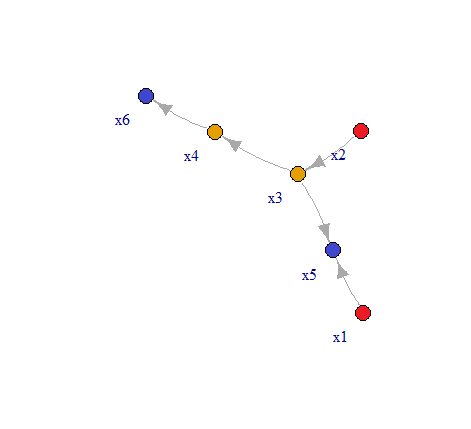
\includegraphics[scale=0.6]{bilder/Sufficient1_Graph.png}
	
%	\caption{Example network. Measured knots $x_5$ and $x_6$, hidden input knots $x_1$ and 
%	$x_2$.}
%	\label{fig:Sufficient1_Graph}
%\end{figure}	
\end{example}